\secnumbersection{PROPUESTA DE SOLUCIÓN}

En el presente capítulo, se explicará la solución propuesta para enfrentar el problema presentado en los capítulos anteriores. Esta se basa, en someter los documentos de la compañía a un proceso de minería y análisis de textos. Para ello, es necesario seleccionar alguna de las metodologías presentadas en el capítulo anterior y definir los experimentos que permitirán extraer la información oculta en dichos activos de la compañía.

\subsection{Metodología}
    La metodología seleccionada para desarrollar este trabajo fue una mezcla entre la propuesta por Kumar (Ver sección 2.2.4) y la propuesta por Google (Ver sección 2.2.5) . Estas metodologías fueron seleccionadas ya que, en primer lugar la propuesta por Kumar entrega la libertad de aplicar cualquier técnica de minería de textos. Por otro lado la guía desarrollada por Google entrega algunos tips interesantes sobre como desarrollar ciertas tareas. Además, según la tabla comparativa (Ver tabla: \ref{table:comparación_metodologías_tm}) estudiada en el
    capítulo anterior, ambas metodología son las que cubren una mayor cantidad de etapas dentro del proceso de minería de textos. 
    
    A continuación, (Ver tabla: \ref{table:My_Methodology})  se puede ver un pequeño resumen de las etapas que serán efectuadas en nuestro proceso de minería de textos. Como se explico más arriba es una mezcla entre la versatilidad de la metodología propuesta por Kumar y algunos de los tips técnicos propuestos por Google.
    
    \begin{table}[h!]
    \centering
    \begin{tabular}{|c|c|c|}
\hline
\textbf{Etapa}                 & \textbf{Metodología} & \textbf{Descripción}                                                                                                                                                                                                     \\ \hline
Obtención de Datos     & Google                & \begin{tabular}[c]{@{}c@{}}Obtener un conjunto de documentos a \\ analizar. Este conjunto debe ser numeroso ya que \\ se debe poder generalizar los resultados encontrados.\end{tabular}                                                       \\ \hline
Preprocesamiento de Textos     & Kumar                & \begin{tabular}[c]{@{}c@{}}Someter los textos a un proceso de \\ preprocesamiento con el fin de eliminar \\ incongruencias y estandarizar los textos.\end{tabular}                                                       \\ \hline
Análisis Exploratorio de Datos & Google               & \begin{tabular}[c]{@{}c@{}}Encontrar métricas que describan \\ el conjunto de datos a estudiar \\ de forma global como por ejemplo:\\  Número de Textos a estudiar, \\ Promedio de palabras por texto, etc.\end{tabular} \\ \hline
Transformación de Textos       & Google               & \begin{tabular}[c]{@{}c@{}}Encontrar una representación numérica \\ para los datos considerando la \\ técnica de minería de textos \\ que se utilizará en la etapa posterior.\end{tabular}                               \\ \hline
Técnicas de Minería de textos  & Kumar                & \begin{tabular}[c]{@{}c@{}}Ejecutar las técnicas de minería de textos \\ seleccionadas anteriormente.\end{tabular}                                                                                                       \\ \hline
Evaluación                     & Kumar                & \begin{tabular}[c]{@{}c@{}}Evaluar el resultado de las técnicas \\ de minería de textos utilizando\\ la opinión de expertos\\  o métricas de desempeño.\end{tabular}                                                     \\ \hline
\end{tabular}
\caption{\label{table:My_Methodology} Descripción de metodología a utilizar} Fuente: Elaboración Propia
    \end{table}

Una vez seleccionada la metodología para trabajar en el proyecto, se deben describir como se desarrollarán cada una de las etapas del proceso de minería de textos. 

\subsection{Proceso de minería de textos}

    En la presente sección se describirán cada una de las etapas del proceso de minería de textos, al cual los documentos fueron sometidos utilizando la metodología seleccionada.
    
\subsubsection{Obtención de datos}
    Antes de iniciar un proyecto de minería y análisis de textos, se deben tener los documentos que serán utilizados a lo largo del trabajo. En el caso de esta memoria, los documentos a analizar son las propuestas técnicas de trabajo de la compañía Hatch. Estos archivos se encuentran almacenados en el sistema de gestión documental de la compañía. Sin embargo, el autor de esta memoria no posee los privilegios para ingresar a dicho sistema, por lo que será tarea del personal de Hatch recolectar los documentos a analizar y entregarlos para la ejecución del proyecto.
    
\subsubsection{Preprocesamiento de Textos}
    Tal como se describió en la sección 2.3, existe una gran cantidad de tareas de preprocesamiento que se deben realizar antes de utilizar cualquier técnica de minería de textos. Considerando la cantidad de documentos que se deben analizar se propone construir un \textit{Normalizador de textos}. Esto con el fin de poder estandarizar de forma rápida y eficiente un número considerable de documentos (Ver figura: \ref{fig:normalizador}). 
    
    \begin{figure}[H]
    \centering
    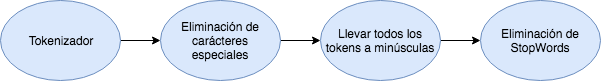
\includegraphics[width=0.8\textwidth]{figures/Normalizador_Textos.png}
    \caption{\label{fig:normalizador} Flujo de preprocesamiento de texto} Fuente: Elaboración Propia.
    \end{figure}
    
    Otra tarea que se debe realizar en esta etapa es el almacenamiento de los documentos en alguna estructura más conveniente para ejecutar las tareas de análisis de forma más rápida y simple. Para ello se propone construir un \textit{json} para cada uno de los documentos a analizar. La estructura de este \textit{json} debe al menos almacenar la siguiente información:
    
    \begin{lstlisting}
    {
        "id": id de la propuesta,
        "proyecto": nombre del proyecto,
        "cliente": cliente de la propuesta,
        "tokens": documento completo tokenizado,
        "keywords_freq": keywords según frecuencia,
        "keywords_pmi": keywords según pmi,
        "estado": estado final de la propuesta ganadora o perdedora,
        "tokens_bigram": bigramas asociados al documento
    }
    \end{lstlisting}
    

\subsubsection{Análisis exploratorio de datos}
    Una vez preprocesados los textos, es importante tener una visión general de los datos que se trabajarán. Esto con el fin de poder tener en cuenta posibles limitaciones en cuanto a conjunto de técnicas a utilizar e información a extraer. Es por esto que antes de realizar cualquier análisis se deben calcular las siguientes métricas:
    
    \begin{itemize}
        \item \textbf{Número de documentos en la muestra}: Número total de documentos a estudiar.
        \item \textbf{Número de clases}: Número de clases definidas a priori dentro del conjunto de documentos a estudiar.
        \item \textbf{Número de muestras por clase}: Número de muestras pertenecientes a cada clase.
        \item \textbf{Número de palabras por documento}: Mediana de palabras por documento.
    \end{itemize}
    
 
\subsubsection{Transformación de textos}
    Una vez preprocesados todos los textos, estos deben representarse de manera numérica para poder ser utilizados dentro de cualquier algoritmo de minería de textos (Ver sección 2.4). Tal como se describió en la respectiva sección, se deben realizar dos pasos para lograr este objetivo: Tokenización y Vectorización. En nuestro caso el proceso de Tokenización será efectuado utilizando bolsas de palabras. Por otro lado dependiendo del algoritmo que se utilizará, las bolsas de palabras serán ponderadas utilizando alguna métrica en particular que será definida al momento de realizar la minería. 
    
    Considerando lo anterior, podemos definir la matriz de documentos $D$ como: La matriz cuyas columnas representan a cada una de las bolsas de palabras encontradas en el corpus, mientras que sus filas representan a cada uno de los documentos pertenecientes al corpus. Considerando esto, el elemento de la matriz $D_{ij}$ será la ponderación de la $j$-ésima bolsa de palabra en el $i$-ésimo documento utilizando alguna métrica en particular.
    
    A modo de ejemplo (Ver tabla: \ref{table:matriz de datos}) se puede ver como lucirá la matriz de documentos.
    
    \begin{table}[H]
    \centering
    \begin{tabular}{c|c|c|l|l|}
    \cline{2-5}
    \textbf{}                                       & \textbf{Bolsa $1$} & \textbf{Bolsa $2$} & \textbf{...............} & \textbf{Bolsa $m$} \\ \hline
    \multicolumn{1}{|c|}{\textbf{Documento $1$}}    &                  &                  &                          &                  \\ \hline
    \multicolumn{1}{|c|}{\textbf{Documento $2$}}    &                  &                  &                          &                  \\ \hline
    \multicolumn{1}{|c|}{\textbf{................}} &                  &                  &                          &                  \\ \hline
    \multicolumn{1}{|c|}{\textbf{Documento $n$}}    &                  &                  &                          &                  \\ \hline
    \end{tabular}
     \caption{\label{table:matriz de datos} Representación de corpus} Fuente: Elaboración Propia.
    \end{table}
    
    
\subsubsection{Proceso de Minería y análisis de textos}
    Una vez realizados todos los pasos anteriores, llega la parte más vital dentro de un proyecto de minería de textos, la cual es seleccionar las técnicas y/o modelos que entreguen la información que se busca. En el caso de esta memoria, el objetivo del proyecto es encontrar los patrones que ayuden a mejorar el proceso de producción de propuestas técnicas. En seguida se desbcriben los experimentos propuestas para lograr dicho objetivo:

    \paragraph{Análisis mediante el uso de Keywords}
    \paragraph*{}
    Como primera aproximación, se deben poder encontrar los elementos que diferencian a una propuesta ganadora de una perdedora, una perdedora de una ganadora y las cosas que estás poseen en común. Para realizar esto, se propone realizar un análisis mediante el uso de KeyWords (Ver sección 2.5.1). El uso de esta técnica, se debe a que debemos realizar un proceso de ''reducción de dimensionalidad´´ para poder, en primer lugar caracterizar cada documento y en segundo lugar poder responder las preguntas planteadas anteriormente, utilizando como elemento a analizar los keywords encontrados para cada documento.  
     
    Tal como se comentó en la sección anterior, se debe seleccionar alguna medida numérica para caracterizar a cada una de las bolsas de palabras dentro del corpus. Para el caso de análisis mediante Keywords se utilizan como medidas: Frecuencia Absoluta y PMI (Ver sección 2.5.1.1).
    
    Una vez realizado el proceso anterior, se espera también poder analizar como los keywords , más relevantes en todo el conjunto de documentos, interactúan dentro de las propuestas ganadoras y perdedoras. Para ello, se propone utilizar un gráfico de dispersión léxica (Ver sección 2.5.4.1.1), el cuál nos permite visualizar como es que ciertos keywords se comportan dentro de documentos ganadores y perdedores. El análisis de esto debe ser capaz de responder preguntas tales como: ¿Existen relaciones entre el uso de Keywords y el resultado de la propuesta?, ¿Es relevante la posición donde se trata cierto keyword dentro de una propuesta?
     
    \paragraph{Modelamiento de Tópicos}
    \paragraph*{}
    Considerando que el experimento anterior caracteriza sólo un documento, es necesario utilizar un algoritmo que pueda realizar un análisis a todo el corpus de manera simultánea. Para ello se utilizará algún algoritmo de modelamiento de tópicos (Ver sección 2.5.2).
    
    Para llevar a cabo un análisis de modelamiento de tópicos, en primer lugar se debe seleccionar algún algoritmo apropiado para realizar esta tarea. En nuestro caso se tienen las opciones de los algoritmos: Latent Dirichlent Allocation (Ver sección 2.5.2.1) y Factorización en matriz no negativa (Ver sección 2.5.2.2) . Si bien ambos algoritmos realizan el trabajo de encontrar los temas latentes que se tratan dentro del corpus de documentos, en el caso de esta memoria se utilizará LDA. Esto, ya que además de entregar los temas tratados por el corpus, el algoritmo entrega una distribución de probabilidades de pertenencia a algún tema en particular para cada uno de los documentos analizados.
    
    Para generar el modelo utilizando LDA, se deben seleccionar tres parámetros en general: $\alpha$ , $\beta$ y $k$. Además para medir la cálidad de un modelo LDA se utiliza el índice de coherencia, por lo que se puede utilizar esta métrica para modelos con distintos $k$ y seleccionar el modelo con el índice más alto. Sólo variamos $k$ ya que en general los valores $\alpha$ y $\beta$ se dejan constantes. 
    
    Luego de tener el modelo seleccionado, este se debe comenzar a explorar. En un principio se deben mostrar los tópicos encontrados por el algoritmo y la definición de estos realizada por el analista. Por otro lado utilizando la composición de temas dentro de cada uno de los documentos es posible responder preguntas como ¿De que temas se habla en propuestas ganadoras y perdedoras? ¿Existen diferencias en la importancia que se le dedica a ciertos temas entre propuestas ganadoras y perdedoras? ¿Que tema predomina en el corpus estudiado?
    
    \paragraph{Clustering usando el resultado de Modelamiento de tópicos}
    \paragraph*{}
    Una vez terminado el proceso de modelamiento de tópicos es posible utilizar la distribución de probabilidades de cada documento, encontrada por LDA, como features de cada documento (Ver tabla:\ref{table:lda_cluster_matrix}). Con esto buscamos encontrar clusters de documentos pero considerando como elementos a agrupar los temas que cada uno de los documentos trata.
    
    \begin{table}[H]
    \centering
    \begin{tabular}{c|c|c|c|c|}
    \cline{2-5}
    \textbf{}                                       & \textbf{\begin{tabular}[c]{@{}c@{}}Probabilidad \\ Tópico 0\end{tabular}} & \textbf{\begin{tabular}[c]{@{}c@{}}Probabilidad\\ Tópico 1\end{tabular}} & \textbf{...............} & \textbf{\begin{tabular}[c]{@{}c@{}}Probabilidad\\ Tópico m\end{tabular}} \\ \hline
    \multicolumn{1}{|c|}{\textbf{Documento $1$}}    &                                                                           &                                                                          &                          &                                                                          \\ \hline
    \multicolumn{1}{|c|}{\textbf{Documento $2$}}    &                                                                           &                                                                          &                          &                                                                          \\ \hline
    \multicolumn{1}{|c|}{\textbf{................}} &                                                                           &                                                                          &                          &                                                                          \\ \hline
    \multicolumn{1}{|c|}{\textbf{Documento $n$}}    &                                                                           &                                                                          &                          &                                                                          \\ \hline
    \end{tabular}
    \caption{\label{table:lda_cluster_matrix} Representación de corpus} Fuente: Elaboración Propia.
    \end{table}
     
     Al ser \textit{clustering} una familia de algoritmos no supervisados (Ver sección 2.5.3) es necesario realizar el proceso de \textit{clustering} con distintos algoritmos y diversas métricas de distancias para encontrar una configuración óptima. En el caso de esta memoria se crearán modelos de clustering aglomerativo y de clustering basado en centroide, utilizando K-Means. Como los datos están dentro del rango $[0,1]$ se debrán probar las distancias: Jensen-Shannon, Euclideana y de Manhattan para cada modelo . Por otro lado, los algoritmos de clustering aglomerativo también deben ser variados con todos los criterios de enlace.
     
     Cuando todos los modelos hayan sido creados se deben comparar utilizando el índice de silhouette, con el fin de encontrar el modelo óptimo de clustering.
     
     Una vez finalizado el proceso de selección de modelo, se debe describir cada uno de los clusters utilizando la \textit{metadata} de cada documento. Esto es, nombre del proyecto, nombre del cliente y tópico dominante en documento, con el fin de encontrar cuales son los documentos que se parecen y relaciones entre estos.
     
     Finalmente para poder comunicar los resultados de forma efectiva, se propone desarrollar una  visualización con los resultados encontrados. La idea es reducir la dimensionalidad de los datos a 2 y luego generar un \textit{scatterplot}. Junto a esto, cada dato debe ser coloreado según el clúster que le corresponda y también debe ser dibujado con alguna forma en particular, dependiendo si el documento es ganador o perdedor.
   
\subsubsection{Evaluación de resultados}
    Una vez terminados todos los experimentos del proceso de minería, se deben comunicar los resultados al principal \textit{stakeholder} del proyecto, en el caso de esta memoria la jefa del equipo de desarrollo de propuestas de la compañía. De esta reunión se espera obtener feedback sobre los estudios realizados, validar las conclusiones extraídas y en conjunto definir los hallazgos útiles que serán incluídos en la guía que se espera obtener como producto final de este proyecto.
     
\subsection{Diseño de Guía}
     Al momento de haber finalizado todo el proceso de minería de textos y con la solución ya validada por el principal \textit{stakeholder} del proyecto, se debe producir una guía que resuma los principales hallazgos que ayuden a mejorar el proceso de producción de propuestas técnicas. La idea es que esta guía sea un punteo de ideas y pequeños tips, que gracias al proceso de minería de texto. fueron posible establecer que de alguna forma hacían a una propuesta tener mayores chances de ganar.
    

    